\documentclass[10pt,twoside,slovak,a4paper]{article}
\usepackage[slovak]{babel}
\usepackage[utf8]{inputenc}
\usepackage{indentfirst}
\usepackage{graphicx}
\usepackage{hyperref}
\usepackage{cite}
\usepackage{url}

\graphicspath{{data}}
\pagestyle{headings}

\title{Paralelný web crawler\thanks{Semestrálny projekt v predmete Metódy inžinierskej práce ak. rok 2023/24, vedenie: Ing. Richard Marko, PhD.}}

\author{Peter Kapusta \\
    \small Slovenská technická univerzita v Bratislave \\
    \small Fakulta informatiky a informačných technológií \\
    \small \texttt{xkapustap@stuba.sk}
}

\begin{document}

\maketitle

\begin{abstract}
    V nasledujúcom článku sa budeme zaoberať využitím paralelných web crawlerov, ako aj problémom optimalizácie (spolu s metódou, ako odľahčiť dopad web crawlerov na jednotlivé webstránky), postupne uvedieme niekoľko riešení, ktoré sa momentálne využívajú a ich spôsoby komunikácie medzi jednotlivými inštanciami. Na konci preberieme dopad paralelných web crawlerov na spoločnosť.
\end{abstract}

\section{Úvod}

Vo všeobecnosti, web crawler je program, ktorý pomocou začiatočného zoznamu odkazov systematicky skenuje web, objavuje webstránky a následne z nich extrahuje informácie a nové odkazy, ktoré vedú k ďalším webstránkam. Cieľom je teda čo najefektívnejšie a najrýchlejšie objaviť čo najväčšie množstvo informácií, ktoré môže neskôr využiť napríklad prehliadač. Hlavnými ťažkosťami sa pri jednoduchých web crawleroch stávajú prehľadávanie HTML kódu a získavanie využiteľných odkazov, čo však pri prehľadávaní a indexovaní celého internetu nie sú jediné komplikácie - vzniká potreba pre sťahovanie a spracovanie masívneho množstva informácií. Pre vyriešenie tohto problému je treba použiť viac ako jeden web crawler. Tu prichádzajú na rad paralelizované web crawlery, ktoré sú výnimočné ich schopnosťou súčasne získavať odkazy z rôznych zdrojov, pomocou osobitných inštancií, bez toho, aby sa prekrývali – tým sa čo najoptimálnejšie využije maximálna rýchlosť sťahovania na danej sieti.

Pri práci s paralelnými web crawlermi je vhodné mať jasný obraz o tom, čo sú vlastne inštancie, ako vyzerajú vzťahy medzi nimi a ako sa medzi sebou prepájajú webstránky, ktorými musia inštancie prechádzať. Pre uľahčenie tohto cieľa si definujeme nasledovné pojmy: Internet môžeme vnímať ako orientovaný graf, ktorého vrcholy sú reprezentované jednotlivými webstránkami a hrany tvoria odkazy medzi nimi \cite{7148493}. Inštancia je proces, ktorý asynchrónne prehľadáva internet a snaží sa nájsť prepojenia, ktoré ho dovedú k novým, ešte neobjaveným informáciám. Úlohou paralelného web crawleru je teda optimálne prechádzať komplexným internetovým grafom, a to pomocou viacerých inštancií, bez toho, aby sa ich cesty krížili.

\paragraph{Historické súvislosti}

Na začiatku boli sekvenčné web crawlery štandardom. Fungujú tak, že prechádzajú hypertextovými odkazmi z jednej webstránky na druhú sériovým spôsobom, pričom získavajú a zbierajú informácie. S exponenciálnym rastom veľkosti a zložitosti internetu sa sekvenčné web crawlery stali neadekvátnymi na spracovanie obrovského množstva webstránok a zvládanie zvyšujúcej sa záťaže na systémy. Ako riešenie tohto problému sa zaviedlo paralelné prehľadávanie webu, ktoré umožňuje rýchlejšie a efektívnejšie vyhľadávanie informácií. Namiesto prechádzania webstránok po jednej, paralelné web crawlery rozdeľujú záťaž prehľadávania medzi viacero inštancií, čo umožňuje súčasné prehľadávanie rôznych webstránok súčasne. Prvým paralelným web crawlerom sa v roku 1994 stal program WebCrawler, ktorý dokázal sťahovať 15 webstránok súčasne. Počet indexovaných webstránok náhle vzrástol z 110 000 na 2 milióny. V roku 1998 vznikol paralelný web crawler Google, ktorý sa odlišoval schopnosťou ohodnotiť relevantnosť webstránok, čo bolo užitočné pri ich následnom zobrazovaní webovým prehliadačom \cite{mirtaheri2014brief}.

\begin{figure}[hbt!]
    \centering
    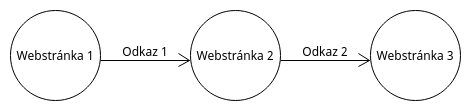
\includegraphics[width=\linewidth]{diagram1.png}
    \caption{Orientovaný graf reprezentujúci vzťah medzi webstránkami}
\end{figure}

\begin{figure}[hbt!]
    \centering
    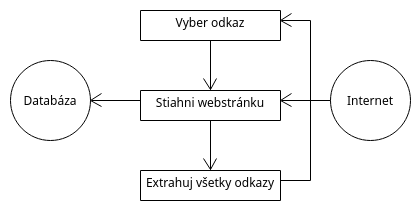
\includegraphics[width=\linewidth]{diagram2.png}
    \caption{Princíp získavania informácií web crawlerom \cite{kausar2013web}}
\end{figure}

\newpage

\section{Porovnanie rýchlosti}

\subsection{Podmienky pri testovaní}

Princíp fungovania paralelných web crawlerov vyžaduje implementáciu, ktorá je rýchla a nenáročná na zdroje. Táto požiadavka sa stáva nevyhnutnosťou, vzhľadom na to, že indexovaný web obsahuje minimálne 5,27 miliárd webstránok \cite{9648837}. Exituje mnoho spôsobov, ako implementovať samotné procesy jednolivých web crawlerov. V tejto časti porovnáme rozdiely vo výkone web crawlerov, ktoré boli vytvorené pomocou procesov, threadov (vlákien) a systémového volania \texttt{epoll} \footnote{Rozhranie poskytované linuxovým jadrom, určené pre oznamovanie I/O udalostí \cite{kerrisk2010linux}}, napísané v programovacom jazyku C++ (vybraný pre rýchlosť a knižnicu \texttt{pthreads}, ktorá je v ňom dostupná) \cite{9648837}.

Pri testovaní implementácií, parametre ako kompilátor (GCC 9.3.0), webserver (operačný systém Ubuntu 20.04 LTS a serverový softvér NGINX), programovací jazyk (C++) a optimizácie pri kompilácii (\texttt{O3} \footnote{Stupeň optimalizácie kompilátora GCC určený pre zvýšenie rýchlosti programu \cite{stallman2009using}}) zostávajú nezmenené. Testy budú spočívať v rýchlosti stiahnutia 132 094 HTML súborov, ktoré sú uložené na serveri, s rozložením veľkostí podľa nasledujúceho grafu \cite{9648837}:

\begin{figure}[hbt!]
    \centering
    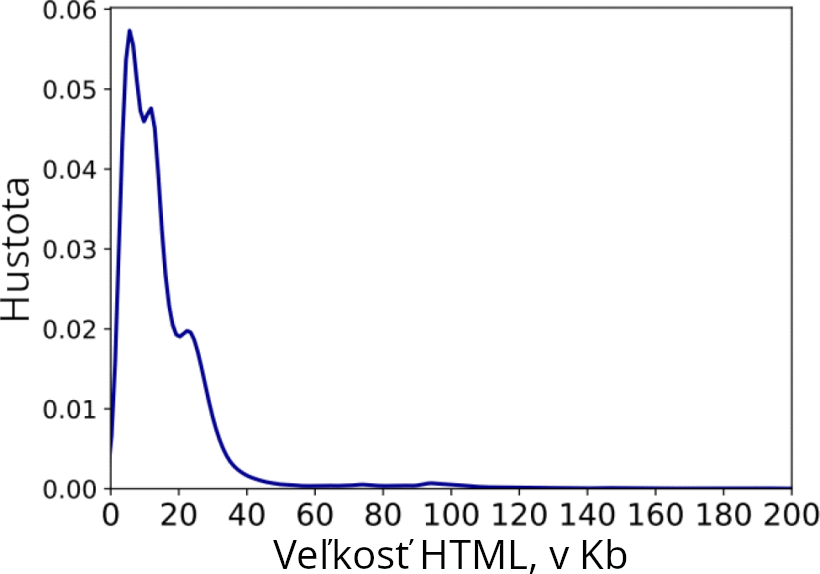
\includegraphics[width=0.75\textwidth]{dataset.png}
    \caption{Graf distribúcie veľkosti HTML súborov. \cite{9648837}}
\end{figure}

\subsection{Podrobnosti implementácií}

Implementácia, ktorá využíva procesy, ich vytvára pomocou systémového volania \texttt{fork} \footnote{Funkcia, ktorá vytvorí z rodičovského procesu nový proces (program sa rozdvojí) \cite{kerrisk2010linux}} - zároveň využíva aj funkcie \texttt{mmap} a \texttt{pthreads} pre zjednodušenie synchronizácie procesov. Počet inštancií pre jednotlivé implementácie bol vybraný tak, aby každá implementácia dovŕšila jej najväčší možný výkon \cite{9648837}.

\subsection{Výsledky}

Z experimentov napokon vyplývajú nasledujúce výsledky (v poradí od najrýchlšej implementácie po najpomalšiu) \cite{9648837}:

\begin{center}
    \begin{tabular}{|l|l|}
        \hline
        Implementácia & Priemerný čas (s) \\ \hline
        Epoll         & 47.9              \\ \hline
        Vlákna        & 49.0              \\ \hline
        Procesy       & 50.1              \\ \hline
    \end{tabular}
\end{center}

Môžeme konštatovať, že systémové volanie \texttt{epoll} je najrýchlejšie v porovnaní s ostatnými testovanými implementáciami. Má aj nevýhody - \texttt{epoll} je dostupný iba na linuxovom jadre (existujú aj alternatívy dostupné v iných jadrách, ako napríklad \texttt{kqueue} na BSD systémoch), rovnako je ho ťažké implementovať, čo môže mať za následok chyby a bezpečnostné problémy. Vlákna majú síce nižší výkon, ale je ich ľahšie naprogramovať. Nakoniec implementácia pomocou procesov je síce najpomalšia, ale pre využitia, kde najvyššia možná rýchlosť nie je na prvom mieste, je postačujúca \cite{9648837}.

\section{Zníženie záťaže na servery}

\subsection{Princíp a implementácia}

40\% prenosu dát internetom je spôsobených web crawlermi, preto by bolo vhodné nájsť riešenie nielen pre sťahovanie čo najväčšieho množstva dát, ale aj pre minimalizáciu opätovného sťahovania webstránok, ktoré už máme v databáze, za účelom aktualizovania ich obsahu. Riešenie spočíva v pridaní súboru UPDATE do každej webstránky na internete. Tento súbor by obsahoval odkazy na adresáry webstránky, kde nastala zmena \cite{mishra2010smart}.

Algoritmus crawlovania \cite{mishra2010smart}:

\begin{enumerate}
    \item Web crawler po prvýkrát navštívi webstránku a stiahne celý adresár (podľa súboru \texttt{robots.txt} \footnote{Súbor, ktorý oznamuje web crawlerom, ktoré časti webstránky môže indexovať})
    \item Pre aktualizáciu databázy web crawler najskôr navštívi súbor UPDATE
    \item Porovná ho s UPDATE súborom z poslednej návštevy webstránky
    \item Ak sú súbory rôzne, web crawler stiahne aktualizované webstránky a uloží ich do databázy
\end{enumerate}

Súbor môže samozrejme pridať len sám vlastník webstránky, čo by vyžadovalo veľkú úroveň koordinácie. Zo strany vlastníkov to má však výhodu - ich server nie je zaplavený žiadosťami o stiahnutie celého adresára, čo znižuje nároky na údržbu. Namiesto toho, aby web crawlery zakaždým sťahovali celý adresár, stačí im overiť si UPDATE súbor. Zo strany web crawlerov vzniká výhoda, že nedochádza k časovo náročnému prehľadávaniu webstránky, ktorej najnovšiu verziu už majú v databáze \cite{mishra2010smart}.

Existencia súboru \texttt{robots.txt} vo veľkom množstve webstránok dokazuje, že je možné takéto riešenie implementovať. Každý web crawler by mal byť schopný prehľadávať HTML kód, a každý vlastník webstránky by mal byť schopný upravovať súbor s HTML kódom, obsahujúci aktualizácie jeho webstránky. Preto by sa mal aj UPDATE súbor skladať z HTML \cite{mishra2010smart}. 

\subsection{Simulácia a výhody}

V experimente bola otestovaná teória stiahnutím najprv celého adresára webstránky, potom pomocou súboru UPDATE s jednou, dvomi a tromi aktualizáciami. Z výsledkov vyplýva, že so súborom s jednou aktualizáciou sa dokopy stiahne 6,5-krát menej webstránok ako bez neho \cite{mishra2010smart}.

Implementácia UPDATE súboru nevyžaduje sťahovanie žiadnych nových programov zo strany vlastníkov a úprava softvéru web crawlerov je minimálna. Je to celkovo veľmi optimálne riešenie problému nadmerného toku web crawlerov na internete \cite{mishra2010smart}.

\section{Moderné riešenia}

\subsection{C-proc}

Paralelné web crawlery sa skladajú z viacerých komponentov, ktoré sa dajú zrealizovať viacerými spôsobmi. Jeden z takých spôsobov je vytvorený pomocou crawlovacích inštancií C-proc. Každý C-proc je oddelený proces, ktorý nezávislo prehľadáva web. Výhodou takejto architektúry je zníženie záťaže na lokálne siete, pretože každý C-proc môže bežať na inej sieti. Jednotlivé inštancie sú ovládané centrálnym programom na správu web crawlerov \cite{sharma2011novel}.

Paralelné web crawlery typu C-proc sa rozdeľujú nasledovne \cite{9645918, sharma2011novel}:

\begin{enumerate}
    \item Viacvláknový server a jeho časti - Koordinujú činnosť jednotlivých inštancií.
        \begin{enumerate}
            \item URL Dispatcher
            \item DNS Resolver
            \item URL Mapper
        \end{enumerate}
        \item Inštancie web crawlerov - Jednotlivé programy C-proc, ktoré sťahujú webstránky
\end{enumerate}

\subsection{Ergate}

Paralelný web crawler Ergate funguje na podobnom princípe ako C-proc, ale odstraňuje problém spoliehania sa na jeden program, ktorý riadi všetky inštancie. Tento cieľ je dosiahnutý pomocou distribuovanej architektúry, zloženej z kontrolného systému a systému na sťahovanie webstránok - každý z týchto systémov sa môže skladať z viacerých inštancií ovládačov a web crawlerov. Jednotlivé časti komunikujú medzi sebou cez MPI \footnote{Message Passing Interface - rozhranie na komunikáciu medzi procesmi} a celok sa nazýva Cluster. Jednou z kľúčových vlastností Ergate je jeho schopnosť rozložiť záťaž na viacero počítačov, čo zvyšuje jeho efektivitu a umožňuje rýchlejšiu extrakciu údajov, čo vedie k výraznej úspore času v porovnaní s tradičnými paralelnými web crawlermi. Využitím distribuovaného prístupu dokáže Ergate spracovať veľké množstvo údajov, vďaka čomu je ideálny na extrahovanie informácií z webstránok s veľkým adresárom \cite{5709184}.

\paragraph{Technológia a ľudia}

V nekonečne sa rozširujúcom internete, paralelné web crawlery hrajú rolu navigátorov, bez ktorých by bolo oveľa ťažšie v globalizovanom svete fungovať. Mohli by sa teda paralelné web crawlery považovať za najdôležitejšiu časť internetu? Technológia poskytuje nástroje a infraštruktúru potrebnú na paralelizáciu, čo umožňuje rozsiahle zhromažďovanie údajov. Ľudia sú však zodpovední za navrhovanie, programovanie a monitorovanie týchto nástrojov, robia kritické rozhodnutia o ich správaní a zabezpečujú, že sú v súlade s etickými zásadami. Ľudská účasť je rozhodujúca pri vytváraní algoritmov, ktoré efektívne rozdeľujú úlohy prehľadávania, spravujú oneskorenia pri extrakcií odkazov s cieľom dodržiavať pravidlá webstránok a vyhýbajú sa nadmernej spotrebe dát na sieti. Paralelné web crawlery môžeme teda považovať za nevyhnutný nástroj na využitie niečoho, čo vzniklo vďaka ľuďom, ktorí vytvorili internet. Sú súčasťou internetu, ale nie sú jeho najdôležitejšou časťou - tvoria jeden celok, ktorého časti sú rovnako dôležité.

\paragraph{Spoločenské súvislosti}

Paralelné web crawlery sa dajú používať aj na osobnú zábavu. Jednotlivci môžu vytvárať paralelné web crawlery na získavanie webstránok a zhromažďovanie mediálneho obsahu, ako sú obrázky, videá alebo súbory GIF, do svojich osobných zbierok. Toto použitie je bežné najmä medzi umelcami, dizajnérmi alebo nadšencami vizuálnych médií, ktorí hľadajú inšpiráciu alebo jednoducho radi budujú osobné archívy \cite{pennock2013web}. Ďalším využitím je zhromažďovanie konkrétnych informácií z viacerých zdrojov. Napríklad vedci a študenti môžu využívať paralelné web crawlery na získavanie relevantných údajov pre svoje štúdie. Umožňujú im analyzovať veľké množstvo údajov a vyvodzovať zmysluplné závery bez toho, aby museli manuálne navštevovať veľký počet webstránok, čo šetrí čas aj námahu.

\section{Záver}

Tento článok poskytol informácie o používaní paralelných web crawlerov a ich optimalizácii, pričom sme sa venovali aj obavám súvisiacim s vplyvom tejto technológie na jednotlivé webstránky. Celkovo sa v článku zdôraznilo, že pri využívaní tejto technológie je dôležité zvážiť jej vplyv na jednotlivé webstránky, ako aj na širšiu spoločnosť.

\newpage

\bibliography{literatura}
\bibliographystyle{unsrt}

\end{document}
